\section{信号的基本概念与数学基础}

这一章主要涉及信号的基本概念与数学基础。

\subsection{信号的概念}

\begin{definition}[信号]
    \bd{信号}是人对物理世界的一种\bd{观察}。
    \bd{观察}是人通过\bd{传感器}对物理世界的一种\bd{测量}。
    \bd{传感器}是把一种物理变化转换成另一种物理变化的装置。
    \bd{测量}是指用一种物理量来表示另一种物理量。

    信号是反映(或载有)信息的物理量,是系统直接进行加工、变换以实现通信的对象。
    信号是信息的表现形式,信息则是信号里所蕴含的内容
\end{definition}

\begin{example}[传感器]
    传感器的种类繁多。例如:
    \begin{enumerate}
        \item 光
            \begin{itemize}
                \item 数码相机:光能产生电信号。
            \end{itemize}
        \item 空气振动
            \begin{itemize}
                \item 麦克风:空气的振动能产生电信号。
            \end{itemize}
        \item 温度
            \begin{itemize}
                \item 热敏电阻:阻值随温度变化。
                \item 热电偶:由对温度反应不同的两种金属制成,温差导致电压。
            \end{itemize}
    \end{enumerate}

    除此之外,还有加速度传感器、压力传感器、流量传感器等。
    值得注意的是,耳朵(图 \ref{fig:ear})就是一种传感器。
    \begin{figure}[H]
        \centering
        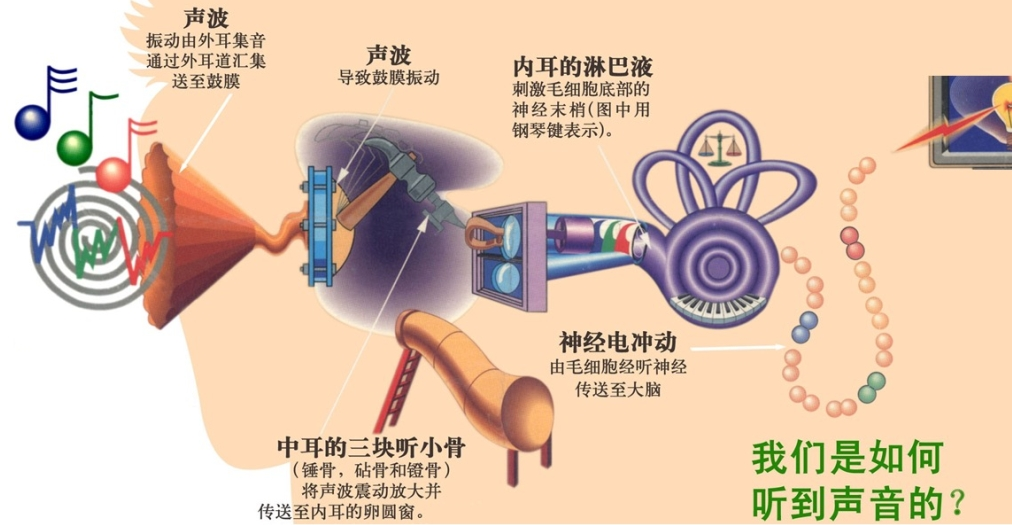
\includegraphics[width=0.5\textwidth]{chap1/img/ear.png}
        \caption{耳朵是一种传感器}
        \label{fig:ear}
    \end{figure}
\end{example}

\begin{definition}[信号处理]
    \bd{信号处理}是对信号进行变换、分析和综合等处理过程的统称。
    信号处理的目的是
    \begin{itemize}
        \item 去伪存真:去除信号中冗余的和次要的成分。
        \item 特征抽取:把信号变成易于进行分析和识别的形式。
        \item 编码解码:把信号变成易于传输、交换与存储的形式(编码),
            或从编码信号中恢复出原始信号(解码)。
    \end{itemize}
\end{definition}

\begin{example}[数字信号处理(DSP)系统]
    由于数字系统的工作具有\bd{可预测性}和\bd{可重复性},
    而模拟系统是由元器件搭建而成的电路,制造误差范围大,
    特性随温度(温度漂移)和时间变化(老化)。
    因此,\bd{数字信号处理(DSP)系统}应运而生。

    DSP 系统的特点有:
    \begin{itemize}
        \item 体积小,功耗低:数字系统通常由集成电路构成,这些电路可以在非常小的尺寸上集成大量的电子元件。这不仅减少了设备的体积,也降低了功耗,这对于移动终端的发展尤为重要。
        \item 有高度的灵活性:数字系统可以通过软件编程来实现多种功能,这使得它们非常灵活。修改程序中的一些语句就能修改系统的行为,而无需改变硬件。
        \item 模拟信号与数字信号的不同:
            \begin{itemize}
                \item 模拟音频以模拟电压的幅度表示声音强弱。
                \item 数字音频是有限数值表示的离散数字序列。
            \end{itemize}
    \end{itemize}
    例如,修改“抽样频率”,就可以改变数字音频音高/音速。
\end{example}

\subsection{信号的描述}

信号的描述有两种方式:数学描述和波形描述。

\begin{definition}[数学描述]
    信号的\bd{数学描述}是指,使用具体的数学表达式,
    把信号描述为一个或若干个自变量的函数或序列的形式。
\end{definition}

\begin{definition}[波形描述]
    信号的\bd{波形描述}是指,按照函数随自变量的变化关系,把信号的波形画出来。
\end{definition}

\begin{note}
    在画波形描述时,需要写清\bd{横纵坐标标识},并\bd{标出原点}。
\end{note}

\begin{example}
    以下是信号的数学描述和波形描述的例子:
    \begin{itemize}
        \item 数学描述:$f(t) = \sin t, x(n) = a^nu(n)$。
        \item 波形描述:$\sa(t) = \frac{\sin t}{t}$ 的示意图如图 \ref{fig:sa-t-wave-description}。
    \end{itemize}
    \begin{figure}[H]
        \centering
        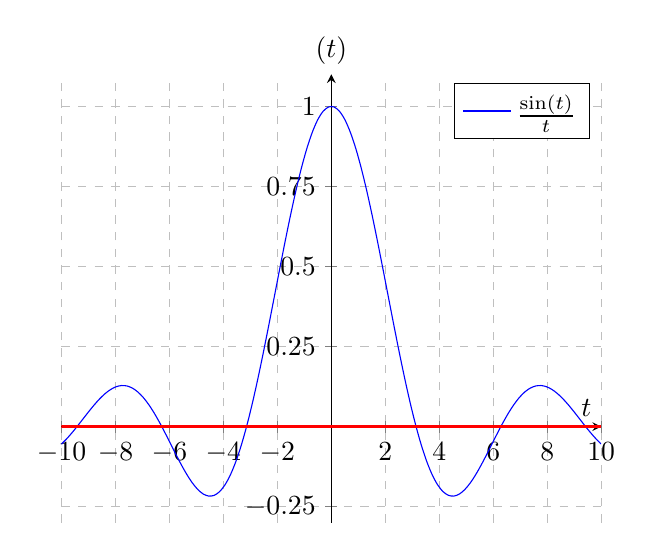
\begin{tikzpicture}
            \begin{axis}[
                axis lines = middle,
                xlabel = {$t$},
                ylabel = {$\sa(t)$},
                ylabel style={at={(rel axis cs:0.5,1)}, anchor=south},
                xmin = -10, xmax = 10,
                ymin = -0.3, ymax = 1.1,
                xtick = {-10,-8,-6,-4,-2,0,2,4,6,8,10},
                ytick distance = 0.25,
                grid = major,
                grid style = dashed,
            ]
            \addplot[domain=-10:10, samples=100, smooth, blue] {sin(deg(x))/x};
            \addlegendentry{$\frac{\sin(t)}{t}$}
            \addplot[domain=-10:10, red, thick] {0};
            \end{axis}
        \end{tikzpicture}
        \caption{$\sa(t) = \frac{\sin t}{t}$ 的波形描述}
        \label{fig:sa-t-wave-description}
    \end{figure}
\end{example}

\begin{example}[时域波形与频谱图]
    时域波形与频谱图如图 \ref{fig:wave-spectrum} 所示。
    \begin{figure}[H]
        \centering
        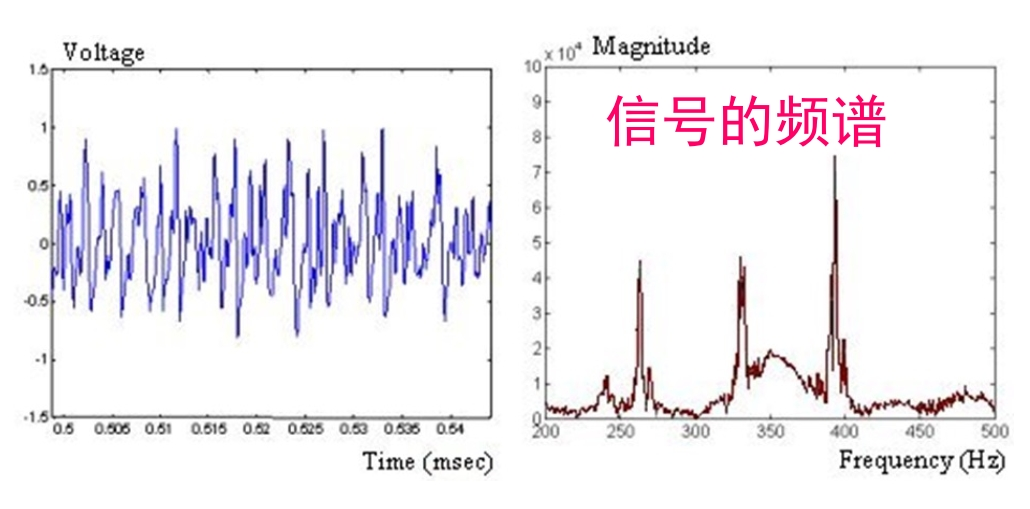
\includegraphics[width=0.5\textwidth]{chap1/img/wave-spectrum.png}
        \caption{左侧为时域波形,右侧为频谱图}
        \label{fig:wave-spectrum}
    \end{figure}
\end{example}

\begin{definition}[确定信号与随机信号]
    任意给定一个自变量的值,如果可以唯一确定其信号和取值,则该信号是\bd{确定信号}。
    否则,如果取值是不确定的随机值,则是\bd{随机信号}。
\end{definition}

\begin{definition}[周期信号]
    如果存在正数 $T$,使得对于任意 $t$ 都有 $f(t) = f(t + T)$,
    则称 $f(t)$ 为\bd{周期信号}。
    周期信号的\bd{周期} $T$ 是使得 $f(t) = f(t + T)$ 成立的最小正数。
\end{definition}

\begin{remark}
    非周期信号可以看做是周期为无穷大的周期信号。
\end{remark}

\begin{example}[正弦信号与余弦信号]
    正弦信号与余弦信号是最常见的周期信号。它们的数学描述如下:
    \begin{itemize}
        \item 正弦信号:$f(t) = K\sin(\omega t + \theta)$。
        \item 余弦信号:$f(t) = K\cos(\omega t + \theta)$。
    \end{itemize}
    其中 $K > 0$ 为振幅,$\omega$ 为角频率,$\theta$ 为初相位。
\end{example}

\begin{example}[$\sa$ 函数]
    $\sa$ 函数的数学描述如下:
    \begin{align*}
        \sa(t) = \frac{\sin t}{t}.
    \end{align*}
    它有以下性质:
    \begin{itemize}
        \item $\sa(t)$ 是偶函数。
        \item $\sa(t)$ 的零点为 $t = k\pi, k \ne 0$。
        \item 过零区间:除原点附近的过零区间宽度为 $2\pi$ 外,
            其他过零区间宽度均为 $\pi$。
        \item $\int_{-\infty}^{0}\sa(t)\D{t} = \int_{0}^{+\infty}\sa(t)\D{t} = \frac{\pi}{2}$,
            $\int_{-\infty}^{+\infty}\sa(t)\D{t} = \pi$。
    \end{itemize}
\end{example}

\begin{note}
    一定要注意,$\sa(t)$ 在 $t = 0$ 处的取值是 $1$,
    而不是 $0$。$\sa(t)$ 的零点不包括 $t = 0$。
\end{note}

\begin{example}[指数信号]
    指数信号是一种常见的非周期信号。它的数学描述如下:
    \begin{align*}
        f(t) = K\mathe^{\alpha t}.
    \end{align*}
    其中 $K > 0$ 为振幅,$\alpha$ 为参数。
    对于 $\alpha$ 的符号而言:
    \begin{itemize}
        \item 若 $\alpha > 0$,则信号随时间\bd{增强}。
        \item 若 $\alpha = 0$,则信号为\bd{直流信号}。
        \item 若 $\alpha < 0$,则信号随时间\bd{减弱}。
    \end{itemize}
    对于 $\alpha$ 的绝对值大小而言:
    \begin{itemize}
        \item 若 $\alpha$ 的绝对值大,则信号变化速度\bd{快}。
        \item 若 $\alpha$ 的绝对值小,则信号变化速度\bd{慢}。
    \end{itemize}
\end{example}

\begin{remark}
    指数信号微分或积分后仍然是指数信号。
\end{remark}

\subsection{欧拉公式}

\begin{definition}[实值信号与复值信号]
    如果信号的取值是实数,则称为\bd{实值信号},简称\bd{实信号}。
    如果信号的取值是复数,则称为\bd{复值信号},简称\bd{复信号}。
\end{definition}

\begin{theorem}[欧拉公式]
    对于任意的 $\theta \in \set{R}$,都有以下的恒等式成立:
    \begin{align*}
        \mathe^{\mathi \theta} = \cos \theta + \mathi \sin\theta.
    \end{align*}

    特别地,当 $\theta = \pi$ 时,有 $\mathe^{\mathi\pi} + 1 = 0$。
\end{theorem}

\begin{proof}
    \nl{(欧拉公式的泰勒级数法证明)} 分别将 $\mathe^x, \sin x, \cos x$ 进行泰勒展开,得:
    \begin{align*}
        \mathe^x &= \sum_{k = 0}^{+\infty}\frac{x^k}{k!}, \\
        \sin x   &= \sum_{k = 0}^{+\infty}\frac{(-1)^kx^{2k + 1}}{(2k + 1)!}, \\
        \cos x   &= \sum_{k = 0}^{+\infty}\frac{(-1)^kx^{2k}}{(2k)!}.
    \end{align*}
    考虑到 $\mathi^2 = -1$,因此可以将 $\cos x$ 和 $\mathi\sin x$ 写成以下形式:
    \begin{align*}
        \cos x &= \sum_{k = 0}^{+\infty}\frac{(\mathi^2)^kx^{2k}}{(2k)!}
                = \sum_{k = 0}^{+\infty}\frac{(\mathi x)^{2k}}{(2k)!}, \\
        \mathi\sin x &= \mathi\sum_{k = 0}^{+\infty}\frac{(\mathi^2)^kx^{2k + 1}}{(2k + 1)!}
                = \sum_{k = 0}^{+\infty}\frac{(\mathi x)^{2k + 1}}{(2k + 1)!}.
    \end{align*}
    故
    \begin{align*}
        \mathe^{\mathi x} & = \sum_{k = 0}^{+\infty}\frac{(\mathi x)^k}{k!} \\
        & = \sum_{k = 0}^{+\infty}\frac{(\mathi x)^{2k}}{(2k)!} + 
            \sum_{k = 0}^{+\infty}\frac{(\mathi x)^{2k + 1}}{(2k + 1)!} \\
        & = \cos x + \mathi \sin x.
    \end{align*}
\end{proof}

\begin{corollary}
    由欧拉公式可得,对于任意的 $\theta \in \set{R}$:
    \begin{align*}
        \sin \theta & = \frac{\mathe^{\mathi\theta} - \mathe^{-\mathi\theta}}{2\mathi}, \\
        \cos \theta & = \frac{\mathe^{\mathi\theta} + \mathe^{-\mathi\theta}}{2}.
    \end{align*}
\end{corollary}

\begin{example}[复值信号的图示]
    如果将 $\mathe^{\mathi \varphi}$ 看成一个复平面上的向量,
    则它的模长为 $1$,辐角主值为 $\varphi$,
    如图 \ref{fig:euler-formula-imaginary-plane} 所示。
    \begin{figure}[H]
        \centering
        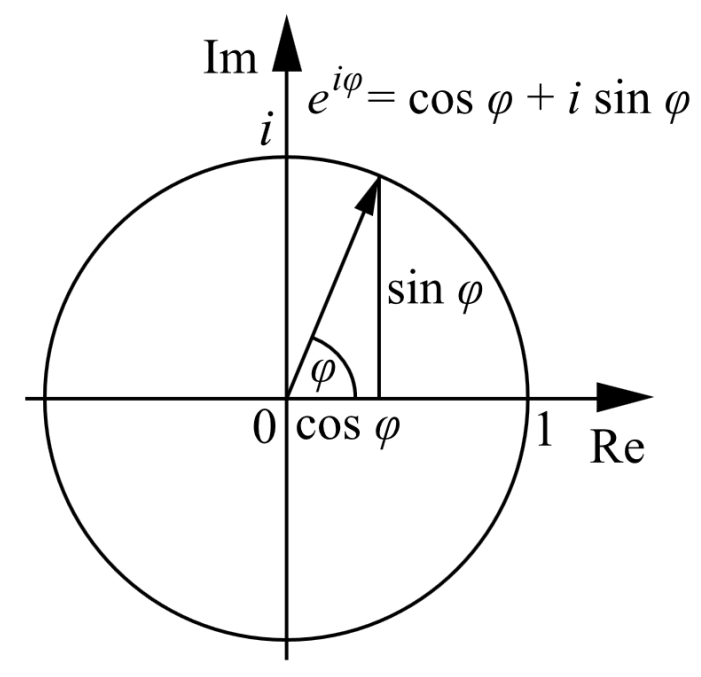
\includegraphics[width=0.5\textwidth]{chap1/img/euler-formula-imaginary-plane.png}
        \caption{$\mathe^{\mathi \varphi}$ 在复平面上的表示}
        \label{fig:euler-formula-imaginary-plane}
    \end{figure}

    如果使 $\varphi$ 随着时间 $t$ 的变化而变化,则画出三维图像(纵轴为时间)
    如图 \ref{fig:euler-formula-imaginary-signals.png} 所示。
    \begin{figure}[H]
        \centering
        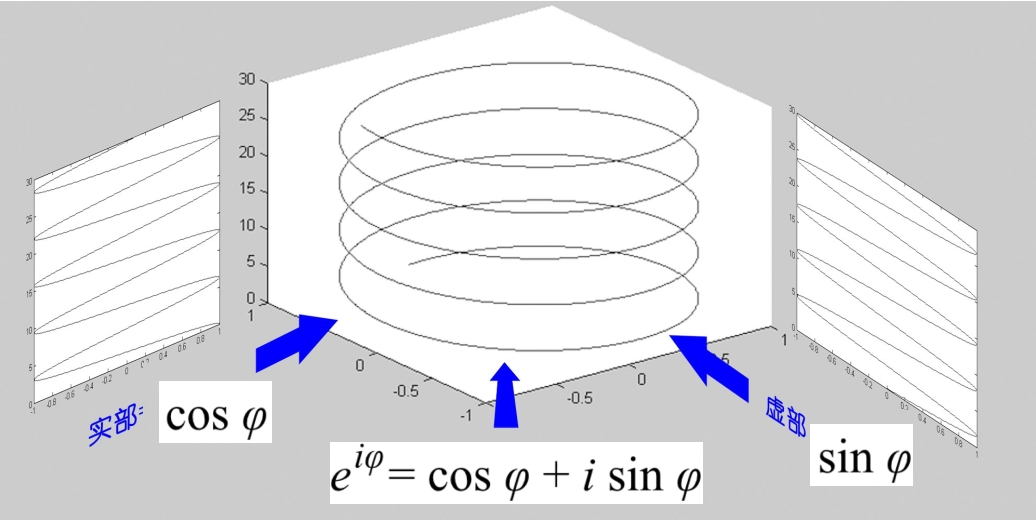
\includegraphics[width=0.5\textwidth]{chap1/img/euler-formula-imaginary-signals.png}
        \caption{$\mathe^{\mathi \varphi}$ 随时间的变化的在三维空间中的轨迹}
        \label{fig:euler-formula-imaginary-signals.png}
    \end{figure}
\end{example}

\begin{example}[复值信号在电磁场中的应用]
    由于电场和磁场互相垂直,所以可以用复值信号的实数部分和虚数部分分别表示电场与磁场信号。
\end{example}

\begin{proof}
    \nl{(欧拉公式的微分法证明)} 设有函数
    \begin{align*}
        f(x) = \frac{\cos x + \mathi \sin x}{\mathe^{\mathi x}}.
    \end{align*}
    则
    \begin{align*}
        \frac{\D{f}}{\D{x}} & = \frac{(-\sin x + \mathi \cos x)\mathe^{\mathi x}
                    - (\cos x + \mathi \sin x)\mathi \mathe^{\mathi x}}
                    {\mathe^{2\mathi x}} \\
        & = \frac{\mathe^{\mathi x}(-\sin x + \mathi \cos x - \mathi \cos x + \sin x)}{\mathe^{2\mathi x}} \\
        & = 0.
    \end{align*}
    因此 $f(x)$ 为常函数,故 $f(x) = f(0) = 1$。
    此即 $\mathe^{\mathi x} = \cos x + \mathi \sin x$。
\end{proof}

\begin{definition}[复指数信号]
    形如 $f(t) = K\mathe^{st}$,其中 $K \in \set{R}, s \in \set{C}$ 为参数,$t \in \set{R}$ 为自变量,
    这样的信号被称为\bd{复指数信号}。
\end{definition}

\begin{property}[复指数信号与正余弦信号之间的关系]
    不妨设 $s = \sigma + \mathi\omega$,其中 $\sigma, \omega \in \set{R}$。则复指数信号
    \begin{align*}
        f(t) & = K\mathe^{st} \\
        & = K\mathe^{(\sigma + \mathi\omega)t} \\
        & = K\mathe^{\sigma t} \cdot \mathe^{\mathi \omega t} \\
        & = K\mathe^{\sigma t} \cdot (\cos \omega t + \mathi \sin \omega t).
    \end{align*}

    固定 $K, \sigma, \omega$ 中的两个,做出第三个关于 $t$ 的变化图像如下:
    \begin{itemize}
        \item 固定 $\sigma = 0.2, \omega = 1$,$K$ 变化:图 \ref{fig:complex-exponential-signal-k-vary}。
        \item 固定 $K = 1, \omega = 1$,$\sigma$ 变化:图 \ref{fig:complex-exponential-signal-sigma-vary}。
        \item 固定 $K = 1, \sigma = 0.2$,$\omega$ 变化:图 \ref{fig:complex-exponential-signal-omega-vary}。
    \end{itemize}
    \begin{figure}[H]
        \centering
        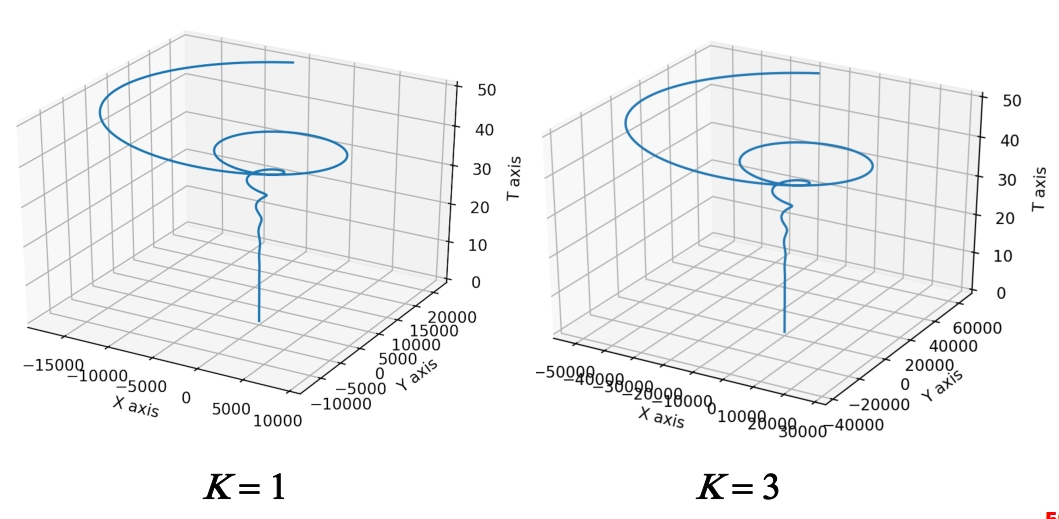
\includegraphics[width=0.5\textwidth]{chap1/img/complex-exponential-signal-k-vary.png}
        \caption{固定 $\sigma = 0.2, \omega = 1$,$K$ 变化}
        \label{fig:complex-exponential-signal-k-vary}
    \end{figure}
    \begin{figure}[H]
        \centering
        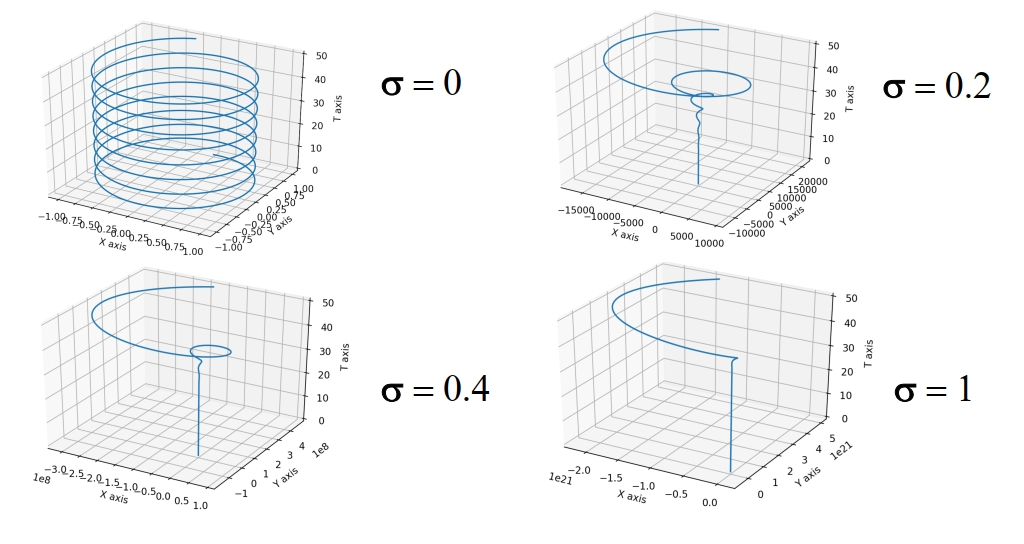
\includegraphics[width=0.5\textwidth]{chap1/img/complex-exponential-signal-sigma-vary.png}
        \caption{固定 $K = 1, \omega = 1$,$\sigma$ 变化}
        \label{fig:complex-exponential-signal-sigma-vary}
    \end{figure}
    \begin{figure}[H]
        \centering
        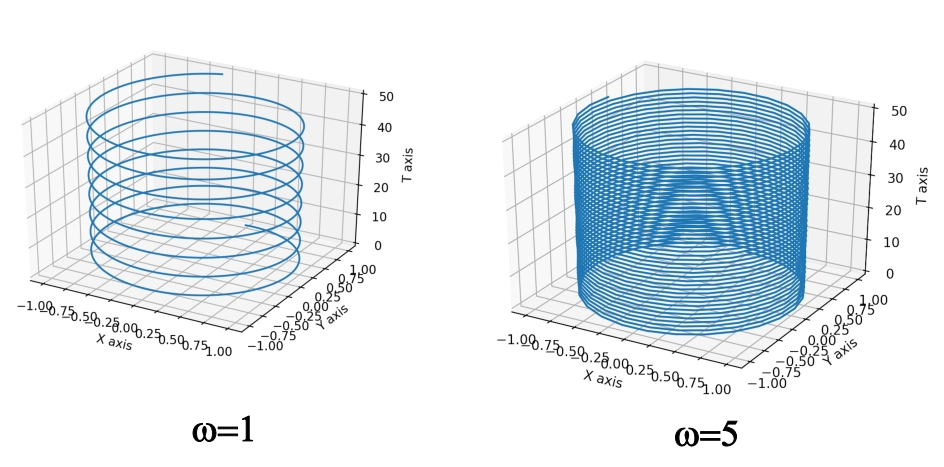
\includegraphics[width=0.5\textwidth]{chap1/img/complex-exponential-signal-omega-vary.png}
        \caption{固定 $K = 1, \sigma = 0.2$,$\omega$ 变化}
        \label{fig:complex-exponential-signal-omega-vary}
    \end{figure}
\end{property}

\subsection{函数分解}

\begin{definition}[正交基]
    设 $V$ 为欧式空间,非零向量 $\alpha_1, \alpha_2, \cdots, \alpha_m \in V$。
    \begin{enumerate}
        \item 如果它们两两正交,则称之为\bd{正交向量组}。
            一个较为显然的事实是,$n$ 维欧式空间中正交向量组所含向量个数 $\le n$。
        \item $n$ 维欧式空间中,由 $n$ 个向量构成的正交向量组称为\bd{正交基}。
        \item 由单位向量构成的正交基称为\bd{标准正交基}。
    \end{enumerate}
\end{definition}

\begin{example}
    在标准欧式空间 $\set{R}^3$ 中,向量组
    \begin{align*}
        \beta_1 = (0, 1, 0),
        \quad \beta_2 = (\frac{\sqrt{2}}{2}, 0, \frac{\sqrt{2}}{2}),
        \quad \beta_3 = (\frac{\sqrt{2}}{2}, 0, -\frac{\sqrt{2}}{2})
    \end{align*}
    是一个标准正交基。这是因为
    \begin{align*}
        \beta_1 \cdot \beta_2 = \beta_1 \cdot \beta_3 = \beta_2 \cdot \beta_3 = 0,
    \end{align*}
    且
    \begin{align*}
        \|\beta_1\| = \|\beta_2\| = \|\beta_3\| = 1.
    \end{align*}
\end{example}

\begin{definition}[正交函数与正交函数集]
    在 $[t_1, t_2]$ 区间上定义的非零函数 $\varphi_1(t)$ 与 $\varphi_2(t)$,
    若满足条件
    \begin{align*}
        \int_{t_1}^{t_2}\varphi_1(t)\varphi_2^*(t)\D{t} = 0,
    \end{align*}
    则称函数 $\varphi_1(t)$ 与 $\varphi_2(t)$ 为在 $[t_1, t_2]$ 区间上的\bd{正交函数}。

    在 $[t_1, t_2]$ 区间上定义的非零函数序列 $\varphi_1(t), \varphi_2(t), \cdots, \varphi_n(t)$,
    其中任意两个函数 $\varphi_i(t)$ 与 $\varphi_j(t)$,均满足条件
    \begin{align*}
        \int_{t_1}^{t_2}\varphi_i(t)\varphi_j^*(t)\D{t} = \begin{cases}
            0, & i \ne j, \\
            k_i, & i = j,
        \end{cases}
    \end{align*}
    其中 $k_i$ 为非零常数,则称函数序列 $\varphi_1(t), \varphi_2(t), \cdots, \varphi_n(t)$
    为区间 $[t_1, t_2]$ 上的\bd{正交函数集}。$n$ 可以为有限值,也可以为正无穷。
\end{definition}

\begin{note}
    在证明正交函数、正交函数集时,需要注意以下几点:
    \begin{itemize}
        \item 在说明正交性时,一定要强调是\bd{在某个区间上}的正交性。
        \item 在说明正交函数集时,除了证明不等两个函数的内积为 $0$ 外,
            还要证明相等的函数的内积不为 $0$。
    \end{itemize}
\end{note}

\begin{example}[三角函数集]
    设 $\omega_0 > 0$,则
    \begin{align*}
        \{1, \cos(\omega_0t + \varphi_1), \cos(2\omega_0t + \varphi_2),
            \cdots, \cos(n\omega_0 t + \varphi_n))\}
    \end{align*}
    是在 $[0, \frac{2\pi}{\omega_0}]$ 区间上的正交函数集。
\end{example}

\begin{proof}
    整个证明分为四部分:
    首先,$1$ 与 $\cos(k\omega_0t + \varphi_k), \quad k = 1, 2, \cdots, n$ 正交。
    \begin{align*}
        \int_{0}^{\frac{2\pi}{\omega_0}}1\cos(k\omega_0t + \varphi_k)\D{t}
        = \int_{0}^{\frac{2\pi}{\omega_0}}\cos(k\omega_0t + \varphi_k)\D{t}
        = 0.
    \end{align*}
    其次,$\cos(k_1\omega_0t + \varphi_{k_1})$ 与 $\cos(k_2\omega_0t + \varphi_{k_2})$, 在 $k_1 \ne k_2$ 的条件下正交。
    \begin{align*}
        & \quad \int_{0}^{\frac{2\pi}{\omega_0}}\cos(k_1\omega_0t + \varphi_{k_1})\cos(k_2\omega_0t + \varphi_{k_2})\D{t} \\
        & = \int_{0}^{\frac{2\pi}{\omega_0}}\frac{1}{2}(\cos((k_1\omega_0t + \varphi_{k_1}) + (k_2\omega_0t + \varphi_{k_2})) + \cos((k_1\omega_0t + \varphi_{k_1}) - (k_2\omega_0t + \varphi_{k_2}))) \\
        & = \int_{0}^{\frac{2\pi}{\omega_0}}\frac{1}{2}(\cos((k_1 + k_2)\omega_0t + \varphi_{k_1} + \varphi_{k_2}) + \cos((k_1 - k_2)\omega_0t + \varphi_{k_1} - \varphi_{k_2}))\D{t} \\
        & = \left(\frac{1}{2(k_1 + k_2)\omega_0}\sin((k_1 + k_2)\omega_0t + \varphi_{k_1} + \varphi_{k_2})
            + \frac{1}{2(k_1 - k_2)}\sin((k_1 - k_2)\omega_0t + \varphi_{k_1} - \varphi_{k_2})\right)\Big|_{0}^{\frac{2\pi}{\omega_0}} \\
        & = 0.
    \end{align*}
    再次,$1$ 与自身不正交。
    \begin{align*}
        \int_{0}^{\frac{2\pi}{\omega_0}}1\cdot 1\D{t}
        = \frac{2\pi}{\omega_0} \ne 0.
    \end{align*}
    最后,$\cos(k\omega_0t + \varphi_k)$ 与自身不正交。
    \begin{align*}
        & \quad \int_{0}^{\frac{2\pi}{\omega_0}}\cos^2(k\omega_0t + \varphi_k)\D{t} \\
        & = \int_{0}^{\frac{2\pi}{\omega_0}}\frac{1 + \cos(2k\omega_0t + 2\varphi_k)}{2}\D{t} \\
        & = \frac{\pi}{\omega_0} + \frac{1}{2}\cdot\frac{1}{2k\omega_0}\sin(2k\omega_0t + 2\varphi_k)\Big|_{0}^{\frac{2\pi}{\omega_0}} \\
        & = \frac{\pi}{\omega_0} \ne 0.
    \end{align*}
    因此,$\{1, \cos(\omega_0t + \varphi_1), \cos(2\omega_0t + \varphi_2), \cdots, \cos(n\omega_0 t + \varphi_n))\}$
    是在 $[0, \frac{2\pi}{\omega_0}]$ 区间上的正交函数集。
\end{proof}

\begin{example}[指数函数集]
    设 $\omega_0 > 0$,则
    \begin{align*}
        \{\mathe^{\mathi n\omega_0t} \mid n \in \set{Z}\}
    \end{align*}
    是在区间 $[-\frac{\pi}{\omega_0}, \frac{\pi}{\omega_0}]$ 上的正交函数集。
\end{example}

\begin{proof}
    任取 $m, n \in \set{Z}$。若 $m \neq n$,则 $\mathe^{\mathi m\omega_0t}$ 和 $\mathe^{\mathi n\omega_0t}$
    在区间 $[-\frac{\pi}{\omega_0}, \frac{\pi}{\omega_0}]$ 上正交,这是因为
    \begin{align*}
        \int_{-\frac{\pi}{\omega_0}}^{\frac{\pi}{\omega_0}}\mathe^{\mathi m\omega_0t}\mathe^{-\mathi n\omega_0t}\D{t}
        = \int_{-\frac{\pi}{\omega_0}}^{\frac{\pi}{\omega_0}}\mathe^{\mathi (m - n)\omega_0t}\D{t}
        = \frac{\mathe^{\mathi (m - n)\omega_0t}}{\mathi (m - n)\omega_0}\Big|_{-\frac{\pi}{\omega_0}}^{\frac{\pi}{\omega_0}}
        = 0.
    \end{align*}
    若 $m = n$,则 $\mathe^{\mathi m\omega_0t}$ 和 $\mathe^{\mathi n\omega_0t}$
    在区间 $[-\frac{\pi}{\omega_0}, \frac{\pi}{\omega_0}]$ 上不正交,这是因为
    \begin{align*}
        \int_{-\frac{\pi}{\omega_0}}^{\frac{\pi}{\omega_0}}\mathe^{\mathi m\omega_0t}\mathe^{-\mathi m\omega_0t}\D{t}
        = \int_{-\frac{\pi}{\omega_0}}^{\frac{\pi}{\omega_0}}1\D{t}
        = \frac{2\pi}{\omega_0} \neq 0.
    \end{align*}
    因此 $\{\mathe^{\mathi n\omega_0t} \mid n \in \set{Z}\}$ 是
    在区间 $[-\frac{\pi}{\omega_0}, \frac{\pi}{\omega_0}]$ 上的正交函数集。
\end{proof}

% \begin{remark}
%     事实上,该函数集在区间 $[-\frac{\pi}{\omega_0}, \frac{\pi}{\omega_0}]$ 上是完备的正交函数集。
% \end{remark}

% \begin{proof}
%     设 $x(t)$ 是在区间 $[-\frac{\pi}{\omega_0}, \frac{\pi}{\omega_0}]$ 上的任意函数。
%     由于 $\{\mathe^{\mathi n\omega_0t} \mid n \in \set{Z}\}$ 是正交函数集,因此
%     \begin{align*}
%         \int_{-\frac{\pi}{\omega_0}}^{\frac{\pi}{\omega_0}}x(t)\mathe^{\mathi n\omega_0t}\D{t} = 0, \quad \forall n \in \set{Z}.
%     \end{align*}
%     由此可得
%     \begin{align*}
%         x(t) = \sum_{n = -\infty}^{+\infty}c_n\mathe^{\mathi n\omega_0t},
%     \end{align*}
%     其中 $c_n = \frac{1}{2\pi}\int_{-\frac{\pi}{\omega_0}}^{\frac{\pi}{\omega_0}}x(t)\mathe^{-\mathi n\omega_0t}\D{t}$。
%     因此 $\{\mathe^{\mathi n\omega_0t} \mid n \in \set{Z}\}$ 是在区间 $[-\frac{\pi}{\omega_0}, \frac{\pi}{\omega_0}]$ 上的完备的正交函数集。
% \end{proof}

\begin{definition}[完备的正交函数集]
    如果在区间 $[t_1, t_2]$ 上,除了正交函数集 $\{\varphi_i(t)\}$ 之外,不存在函数 $x(t)$,
    满足 $0 < \int_{t_1}^{t_2}x(t)x^*(t)\D{t} < +\infty$,使得
    \begin{align*}
        \int_{t_1}^{t_2}x(t)\varphi_i^*(t)\D{t} = 0, \quad \forall i,
    \end{align*}
    则称此正交函数集 $\{\varphi_i(t)\}$ 为区间 $[t_1, t_2]$ 上的\bd{完备的正交函数集}。
\end{definition}
